\section{Experimental Setup}

\subsection*{Circuit components}
    \begin{enumerate}
        \item A variable transformer
        \item 4 junction diodes
        \item A.C. power supply
        \item A zener diode ($V_\text{breakdown} = 5.6$ V)
        \item Current limiting resistors
        \item Load resistors
        \item Capacitor (100$\mu$ F)
        \item Multimeters
        \item Connecting wires
        \item Breadboard
    \end{enumerate}

    \subsection*{Circuit Diagram}
    \begin{figure}[H]
        \centering
        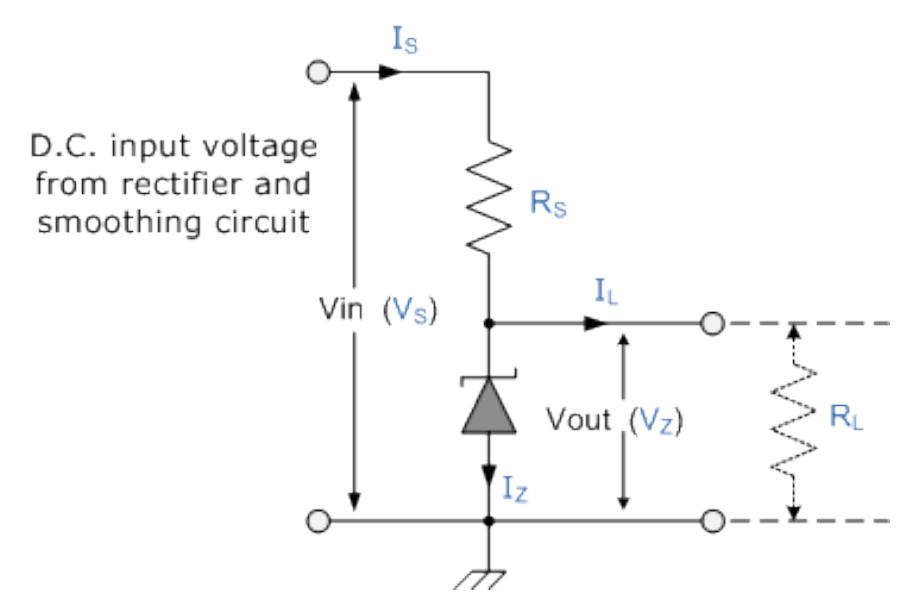
\includegraphics[width=1\columnwidth]{images/f1.png}
        \caption{Circuit diagram for the setup.}
        \label{fig:1}
    \end{figure}

\section{Data Analysis}
\subsection*{Load Regulation}
    The plot for the load voltage vs load resistance looks like this.

    \begin{figure}[H]
        \centering
        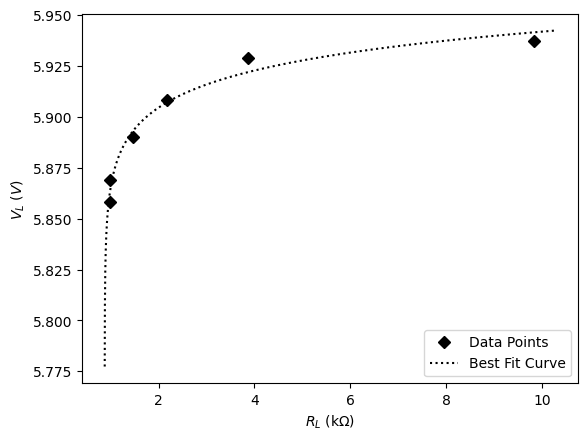
\includegraphics[width=0.8\columnwidth]{images/g1.png}
        \caption{Output voltage vs load resistance plot for a fixed input current}
        \label{fig:2}
    \end{figure}

    As you can see, the load voltage increases rapidly with increases in load resistance and then stabilises after certain value of $R_L$. 
    
    At $R_L = \infty$ (no load current), $V_{NL} = 5.938$ V. For this setup, load voltage with full load (maximum load current) is $V_{FL} = 5.858$ V.

    Therefore, percentage load regulation (Eq. 6) can be calculated as,
    \begin{align*}
        \text{Load Regulation} &= \frac{5.938-5.858}{5.858}\times 100\%\\
        &=1.366\%
    \end{align*}

    Additionally, we can plot $V_L$ vs $I_L$.

    \begin{figure}[H]
        \centering
        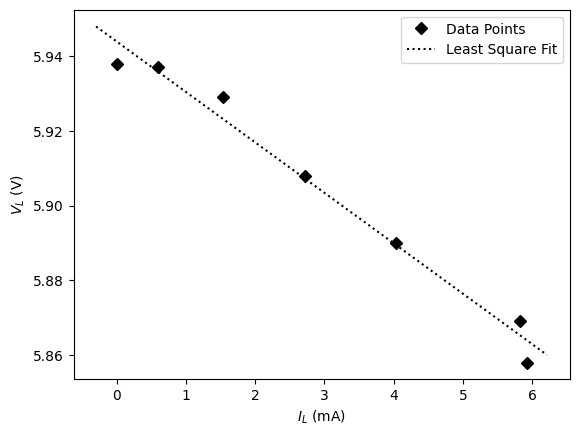
\includegraphics[width=0.8\columnwidth]{images/g2.png}
        \caption{Output voltage vs output current plot for different values of loads ($R_L$) for a fixed input voltage}
        \label{fig:2}
    \end{figure}

    As current across the load, $I_L$ decreases (for increasing values of load resistance), the current across the zener diode, $I_Z$ increases to keep $I_S$ constant. Thus, there is no change in voltage across $R_S$ and thus $V_L$ ideally remains constant. In reality,  due to the presence of output impedance or wire resistances, the voltage at the power supply pin on the load device simply behaves according to Ohm’s Law. To fix this, feedback loop control systems are used in real circuits.

\subsection*{Line Regulation}
    With the load resistance fixed at $R_L = 2.179\,\text{k}\Omega$, plot $V_L$ vs $V_i$ (Fig. 4). 

    \begin{figure}
        \centering
        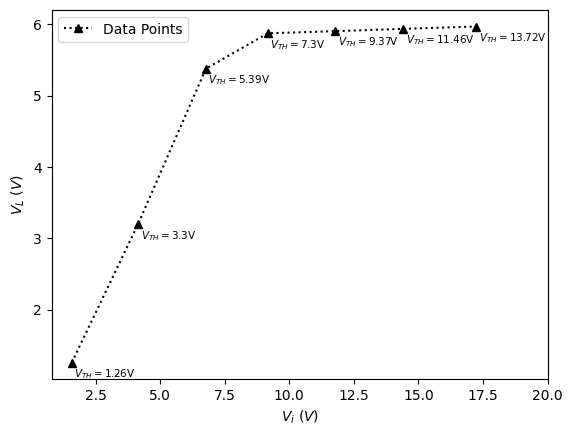
\includegraphics[width=0.9\columnwidth]{images/g3.png}
        \caption{Output voltage vs input voltage for a fixed load resistance ($R_L=2.179$ k$\Omega$)}
        \label{fig:3}
    \end{figure}

    As the load input voltage increases, we can see that load voltage also increases until it becomes roughly constant after a certain $V_i$. We can observe is this point is right after $V_{TH}$  crosses the zener breakdown voltage (5.6V). Hence, we can take $V_{LL}$ as the output voltage after $V_{TH}$ just crosses the zener breakdown, i.e. $V_{LL} = 5.875$ V (at $V_{TH}=7.299)$.

    Additionally, for this setup, $V_{HL} = 5.970$ V (at $(V_i)_\text{max}=17.24$ V. Therefore, percentage line regulation (Eq. 7),
    \begin{align*}
        \text{Line Regulation} &= \frac{5.970-5.875}{5.875}\times 100\%\\
        &=1.617\%
    \end{align*}

     \begin{figure}
        \centering
        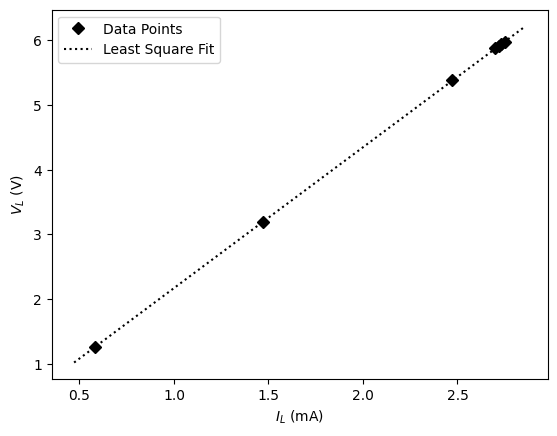
\includegraphics[width=0.9\columnwidth]{images/g4.png}
        \caption{Output voltage vs output current for a fixed load resistance}
        \label{fig:4}
    \end{figure}

    Additionally from Fig. 5, we can see that $V_L$ and $I_L$ increase proportionally (following Ohm's law), until $V_L$ roughly stabilises (after $V_i$ crosses the zener breakdown). After that the value of $I_L$ is also roughly constant. 

\section{Error Analysis}
For percentage load regulation, from Eq. (6), propagated error can we written as

\begin{align*}
    \frac{\Delta LR_\text{load}}{LR_\text{load}}&= \sqrt{\left(\frac{\partial LR_\text{load}}{\partial V_{NL}}\Delta V_{NL}\right)^2+\left(\frac{\partial R_\text{load}}{\partial V_{FL}}\Delta V_{FL}\right)^2}\\
    &=\sqrt{\left(\frac{\Delta V_{NL}}{V_{FL}}\right)^2+\left(\frac{- V_{NL}\Delta V_{FL}}{V_{FL}^2}\right)^2}\\
    &\implies \Delta LR_\text{load} =0.024\%
\end{align*}

Using $\Delta V_{FL} = \Delta V_{NL} = 0.001$ V, the least count of the multimeter. Similarly, error in percentage line regulation can be calculated using Eq. (7),

\begin{align*}
    \frac{\Delta LR_\text{line}}{LR_\text{line}}&= \sqrt{\left(\frac{\partial LR_\text{line}}{\partial V_{HL}}\Delta V_{HL}\right)^2+\left(\frac{\partial R_\text{line}}{\partial V_{LL}}\Delta V_{LL}\right)^2}\\
    &=\sqrt{\left(\frac{\Delta V_{HL}}{V_{LL}}\right)^2+\left(\frac{- V_{LL}\Delta V_{LL}}{V_{LL}^2}\right)^2}\\
    &\implies \Delta LR_\text{line} =0.017\%
\end{align*}